\subsection{Rectangle-line picking}
\label{sec:rectangle_line}


Here we consider choosingp lines from a rectangle with side lengths
$a$ and $b$, which we order $a \leq b$ without loss of generality. 
We could also describe the problem by the aspect ratio of the
rectangle, i.e., $a \!: \!b$.

Figure~\ref{fig:rect_eg} shows a 2D example, Figure~\ref{fig:rect_pdf}
shows the PDF for one rectangle, and Figure~\ref{fig:rect_pdf_var}
shows the PDFs for various rectangles chosen such that $\sqrt{a^2 +
  b^2} = 1$ to allow comparison (the choice means that the PDFs have
the same support).

\begin{figure}[tbp]
  \begin{center}
    \subfloat[\label{fig:rect_eg}Rectangle example.]{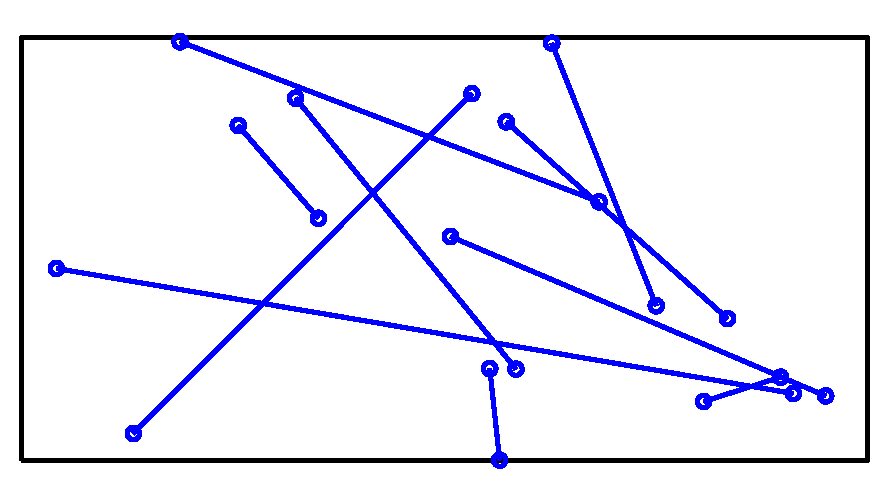
\includegraphics[width=0.28\columnwidth]
          {../Matlab/Plots/LinePicking_eg_rect.eps}} 
    \hspace{6mm}
    \subfloat[\label{fig:rect_pdf}PDF of a rectangles with aspect
    ratio 1:1.2 showing the three regions.]{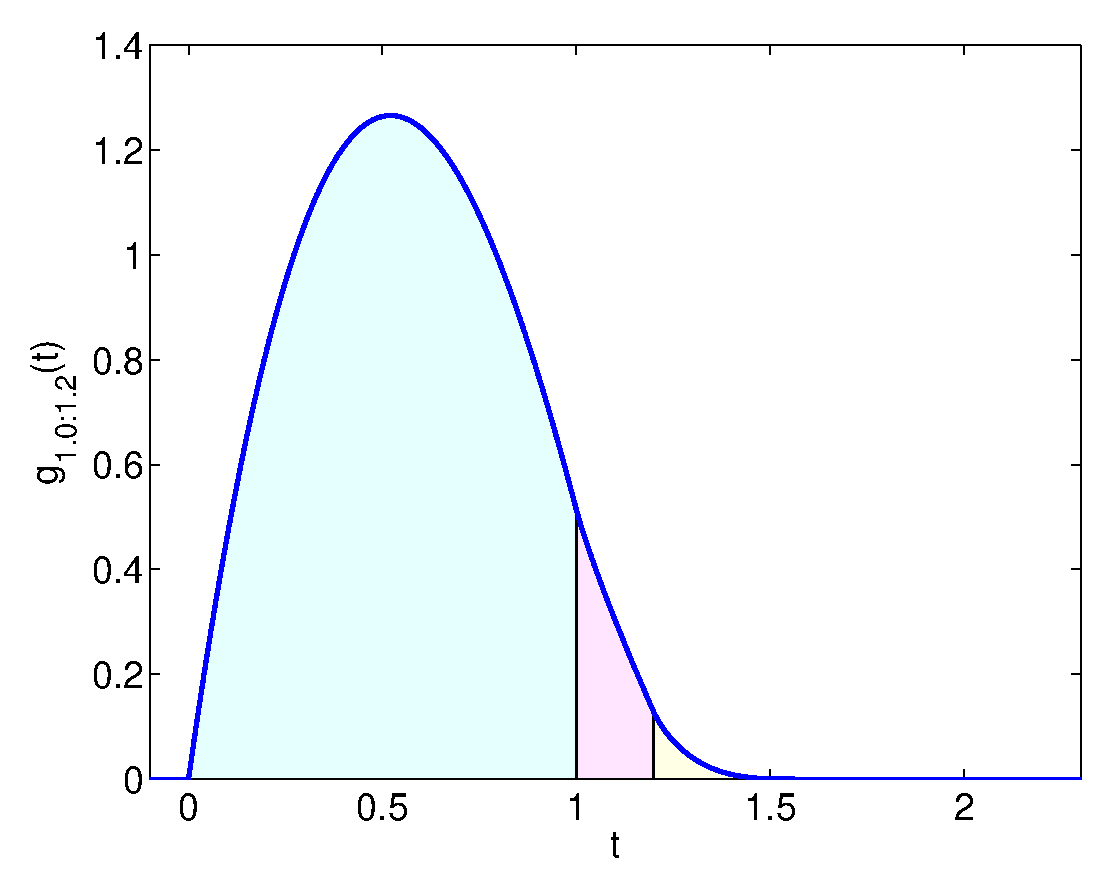
\includegraphics[width=0.35\columnwidth]
          {../Matlab/Plots/LinePicking_plot_rect_regions.eps}}
    \subfloat[\label{fig:rect_pdf_var}PDF of rectangles with various aspect
    ratios.]{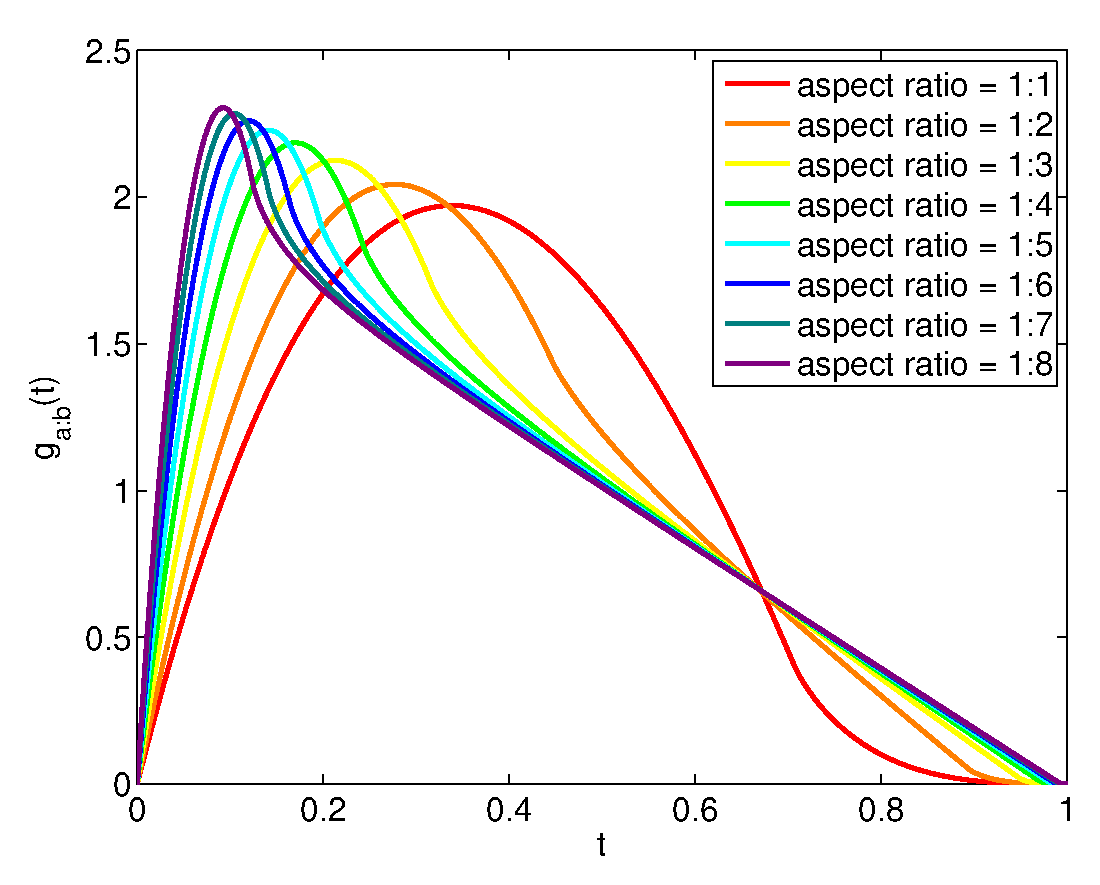
\includegraphics[width=0.35\columnwidth]
          {../Matlab/Plots/LinePicking_plot_rect.eps}}
    \caption{The rectangle-line picking problem.}
  \end{center} 
\vspace{-4mm}
\end{figure}

\subsubsection{PDF}

The PDF for the rectangle is given in \cite[Theorem
2.4.4]{mathai_geom} and \cite[Theorem 2]{b.ghosh51:_random_rect}
\begin{equation}
  g^{\rm rect}_{a,b}(t) = \frac{4 t}{a^2 b^2} \phi_{a,b}(t),
  \label{eqn:rectangle}   
\end{equation}
where
\begin{equation}
  \phi_{a,b}(t) = \left\{
    \begin{array}{ll}
      \frac{ab \pi}{2} - (a+b) t + \frac{t^2}{2}, 
         & \mbox{ for } t \leq a, \\
      a b \sin^{-1} (a/t) - \frac{a^2}{2} - b t + b\sqrt{t^2 - a^2},
         & \mbox{ for } a \leq t \leq b, \\
      a b \left[ \sin^{-1} (a/t) - \sin^{-1} \sqrt{1 - \frac{b^2}{t^2}} \right]
        - \frac{a^2 + b^2 + t^2}{2} 
        + a\sqrt{t^2 - b^2}+ b\sqrt{t^2 - a^2},
         & \mbox{ for } b \leq t \leq \sqrt{a^2 + b^2}, \\
      0,
         & \mbox{ otherwise}, \\
    \end{array} \right. 
\end{equation}
where the rectangle has sides of length $a \leq
b$. Figure~\ref{fig:rect_pdf} shows these for various cases, chosen
such that $\sqrt{a^2 + b^2} = 1$ to allow comparison. We label these
rectangles by their aspect ratio $a: b$.

This is a rather complicated expression, but is easily evaluated
numerically.  Naldi \cite{m.naldi05:_connec_of_waxman_graph}
approximated this expression with a $\beta$ function, though given the
requirements to numerically evaluate that function there hardly seems
any advantage, though we shall see later that this would have been
completely appropriate if the region have been a circle.

We can also see that for longer, thinner rectangles, the PDF is
comprised of two main segments: (i) a part approximating the shape of
that for the square (though compressed into a short range of values of
$t$), and (ii) an almost straight component, similar to the PDF for
line-line picking problem. The reasons for this also seem relatively
intuitive. 

We can calculate the limit as $a \rightarrow 0$ to see the PDF for the
line-line picking problem.  We keep $a^2 + b^2 = L^2$ so that the
support of the PDF remains constant.  As $a \rightarrow 0$, we only
need consider the case $a \leq t \leq b$, where
\begin{eqnarray}
    g^{\rm rect}_{a,b}(t)
        & = & \frac{4 t}{a^2 b^2} 
                  \left[ a b \sin^{-1} (a/t) - \frac{a^2}{2} - b t + b\sqrt{t^2 - a^2} \right] , \nonumber \\
        & \simeq & \frac{4t }{a b} \sin^{-1} (a/t)
                   - \frac{2 t}{b^2}
                    + \frac{4 t}{a^2 b^2} \left[ -b t + b t - \frac{b a^2}{2 t} \right] , \nonumber \\
        & \simeq & \frac{2}{b}
                   - \frac{2 t}{b^2}, 
\end{eqnarray}
where we have used the following Taylor series around $x=0$, dropping
the higher order terms:
\[ \sin^{-1}(x) = x + \frac{x^3}{6} + \cdots, 
   \mbox{ and }
   \sqrt{t^2 - x^2} = t - \frac{x^2}{2t} - \frac{x^4}{8 t^3} \cdots .
\]
The result just returns to the line-line picking PDF.

\subsubsection{CDF}


\subsubsection{Moments}

Ghosh \cite{b.ghosh51:_random_rect} gives the first four moments of
the line-length distribution for the rectangle.
\begin{eqnarray}
  \label{eq:rect_moments} 
  \alpha_1 & = & \frac{1}{6} \left[ 
                        \frac{b^2}{a} \cosh^{-1}\left( M/b \right) +
                        \frac{a^2}{b} \cosh^{-1}\left( M/a \right) 
                 \right]
                  + \frac{1}{15} \left[ \frac{a^3}{b^2} + \frac{b^3}{a^2} \right]
                  - \frac{M}{15} \left[ \frac{a^2}{b^2} + \frac{b^2}{a^2} -3 \right],
\\
  \alpha_2 & = & \frac{1}{6} M^2, \\
  \alpha_3 & = & \frac{1}{20} \left[ 
                        \frac{b^4}{a} \cosh^{-1}\left( M/b \right) +
                        \frac{a^4}{b} \cosh^{-1}\left( M/a \right) 
                 \right]
                  + \frac{2}{105} \left[ \frac{a^5}{b^2} + \frac{b^5}{a^2} \right]
                  - \frac{2M}{105} \left[ \frac{a^4}{b^2} + \frac{b^4}{a^2}\right]
                        - \frac{5}{84} M^3, 
\\
  \alpha_4 & = & \frac{1}{15} a^4 + \frac{1}{18} a^2 b^2 + \frac{1}{15} b^4,
\end{eqnarray}
where $M = \sqrt{a^2 + b^2}$, from which we can derive the special
cases of the square and line (though these can also be derived
directly). Obviously central moments such as mean, and variance, etc.,
can be derived from these. 
